
\section{IoT \& Big Data Platform}
\label{sec:platform}

Challenges of WAZIUP will be tackled using an open IoT-big data platform with affordable sensors connected through an IoT-Cloud open platform.
This platform will also make use of mobile phones and real-time processing to empower users and deliver the needed services.
The project will not develop any new IoT/Big Data software platform, but, rather exploit the existing solutions and adapt them for the purpose. Hereafter a compact list of core technical functionalities encompassed by the platform:

\begin{itemize}
   \item \emph{Cloud-based real-time data collection combined with analytics and automation software:} thus, the platform will offer cost-effective solutions for aggregating different machines and sensor types to engender efficiency, smart automation and optimization in the rural context.
   \item \emph{Intelligent analytics of sensor and device data:} studied in order to optimize for performance of the rural workplace, detect potential outages, and finally reduce overall maintenance costs.
   \item \emph{Integration to 3rd parties' platform:} enables customers' benefit of scaling fast and easy.
   \item \emph{PaaS (Platform-as-a-Service) provider:} WAZIUP will provide to business clientele with independently maintained platform upon which their web application, services and mobile applications can be built.
\end{itemize}

\subsection{Functional overview}
This section presents the functional view of the architecture. 

\begin{figure}[h!]
\centering
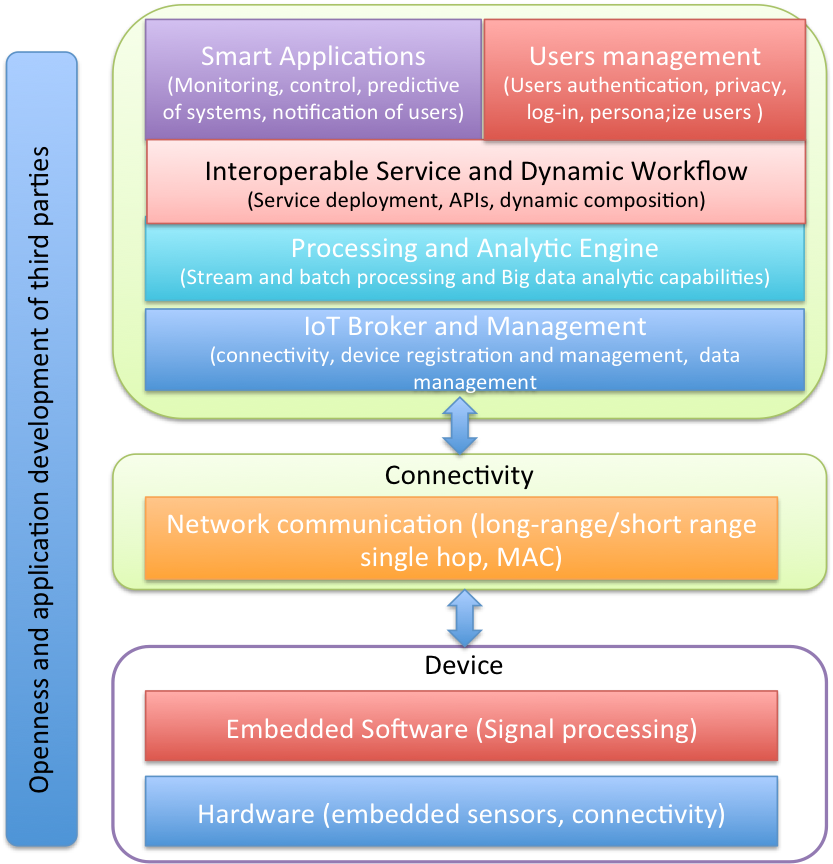
\includegraphics[width=0.7\textwidth]{figs/functional.png}
\caption{Functional overview of WAZIUP}
\label{fig:func}
\end{figure}

The Figure~\ref{fig:func} displays the functional overview of WAZIUP.
The topmost block represents the Cloud platform, the middle one is the network connectivity while the bottom one is the local deployment, including gateway and sensors.
The following functional domains have been identified:

\begin{itemize}
  \item \emph{Application platform}
	Application writing, deploying, hosting and execution.
  \item \emph{Stream and data analytic}
	Data brokering, stream processing and data analytics.
  \item \emph{Users Management}
	Management of the identification, roles and connections of users.
  \item \emph{Gateway, sensors and networks}
	The IoT connectivity, the sensors data and metadata.
  \item \emph{Security and privacy}
	The anonymisation of the data, securisation of the transmissions.
  \item \emph{Platform Management}
	Status of the components, deployment of the platform
\end{itemize}

Based on the functional domains, actors have been identified. 
An actor is either a physical person or an external system. 
There are five actors: the developer, the data provider, the sensor owner, the application user and finally the administrator.

\paragraph{Developer}
The developer uses WAZIUP platform to compile and deploy his application which is then hosted on the platform and accessible. He must collect requirements for WAZIUP app, design the app architecture and then realize, deploy and maintain it into the WAZIUP Platform. 

\paragraph{The data provider}
The data provider is a third party owning an internet API to which WAZIUP is connecting in order to retrieve data. It must be able to integrate a third party API, control and maintain the API. 

\paragraph{The sensor owner }
The sensor owner is installing and deploying the sensors in the field, and then registering them on the WAZIUP platform. Sensor data becomes available to applications after the sensors configuration.

\paragraph{The application user}
The application user is accessing the application developed by the Developer and deployed on WAZIUP. For that he must register with WAZIUP and he is asked to provide feedback on app. 

\paragraph{The administrator}
The administrator manages and configure the platform; and administrates the users. He also control the resources usage. 

\subsection{IoT platform}

\subsubsection{IoT architecture overview}

WAZIUP IoT platform architecture is presented in Figure~\ref{fig:iotarchi}.
It has three main layers: device layer, gateway layer and the cloud layer.

\begin{figure}[h]
\centering
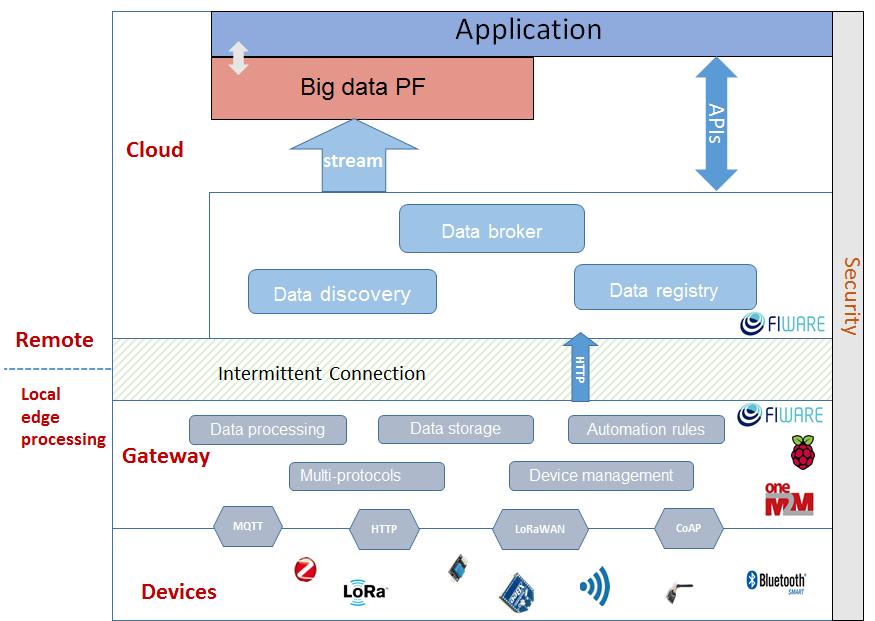
\includegraphics[width=\textwidth]{figs/iotarchi.png}
\caption{IoT platform architecture}
\label{fig:iotarchi}
\end{figure}

\begin{itemize}
  \item \emph{The device layer}
    It includes IoT sensors and actuator that are able to communicate each on its protocol (MQTT, CoAP, HTTP, LoRAWAN) with the gateway. 
It a constraint and autonomous device. 
Considering the project circumstances it has to be low cost and doesn’t consume much power.
  \item \emph{The gateway layer}
  The gateway is a key component in our architecture since it ensure a secure bidirectional communication between the Iot devices and the cloud services.
 It interfere with various kind of devices: getting the data from sensors and sending commands to actuators.
  It has to be multi-protocol in order to be able to support diverse devices and it need to have device management capabilities.
Since the connection is intermittent in our project, it is mandatory that the gateway is able to manage automation rules (for example some event processing), to store data locally and to have low speed internet connectivity (2G: GPRS, EDGE).
  \item \emph{The cloud layer}
  Our cloud main component are: the Data broker, the data registry and the data discovery. 
Data broker is the key component of the IoT cloud services, it is based on publish/ subscribe mechanism to ensure data transfer from different producers to their respected consumers.
Data registry contains the virtual representation of devices (the data and the meta-data)
Finally, data discovery is responsible of querying the data.
\end{itemize}

\subsection{Big Data Platform}

The Big Data platform will allow developers to proceed data analysis with cutting-edge tools. 
Based on the state-of-the-art analysis, we will choose the best fitted tools to analyze the data coming from IoT sensors. 
Some specificities will be mandatory, such as the capacity to proceed streaming analysis. 
To make some predictions and to help to decision making, we will need some machine learning capacities, with dedicated algorithms libraries or independant tools.
We will select the Big Data platform analytics tools based on each specific use case which will require different analysis. 
All the tools will be available on the big data platform, to proceed analysis directly on WAZIUP cloud, or to be installed on a local machine, with a manifest to help deploying the analysis.




